\chapter{Appendix A}

 \subsection{Wave-data check}
 
Estimation of fetch-limited Waves; Method of Verhagen and Young: \\
$ \tilde{H}=\tilde{H}_{\infty}[tanh(k_1 \tilde{F}^{m_1})]^p $ with $ \tilde{F}= \frac{g F}{U_{10}^2} $ and $H_{m0} = \frac{\tilde{H} U_{10}^2}{g} $ \\
The input:
\begin{itemize}
\item $\tilde{H}_{\infty}= 0.24 $
\item $k_1= 4.41*10^{-4} $
\item $ m_1= 0.79 $
\item $p= 0.572 $
\item $F= 1000 km $
\item $U_{10}= 20 \frac{m}{s} $
\end{itemize}
 and the results:
 \begin{itemize}
 \item $\tilde{F}=25000 $
 \item $\tilde{H}= 0.22 $
 \item $H_{m0}= 8.8 m $
 \end{itemize}
 8.8 m is the maximum possible wave hight according to the fetch length and the Young/Verhagen method of dimensionless fetch.
 \\
\begin{figure}[H]
\center
\fbox{
 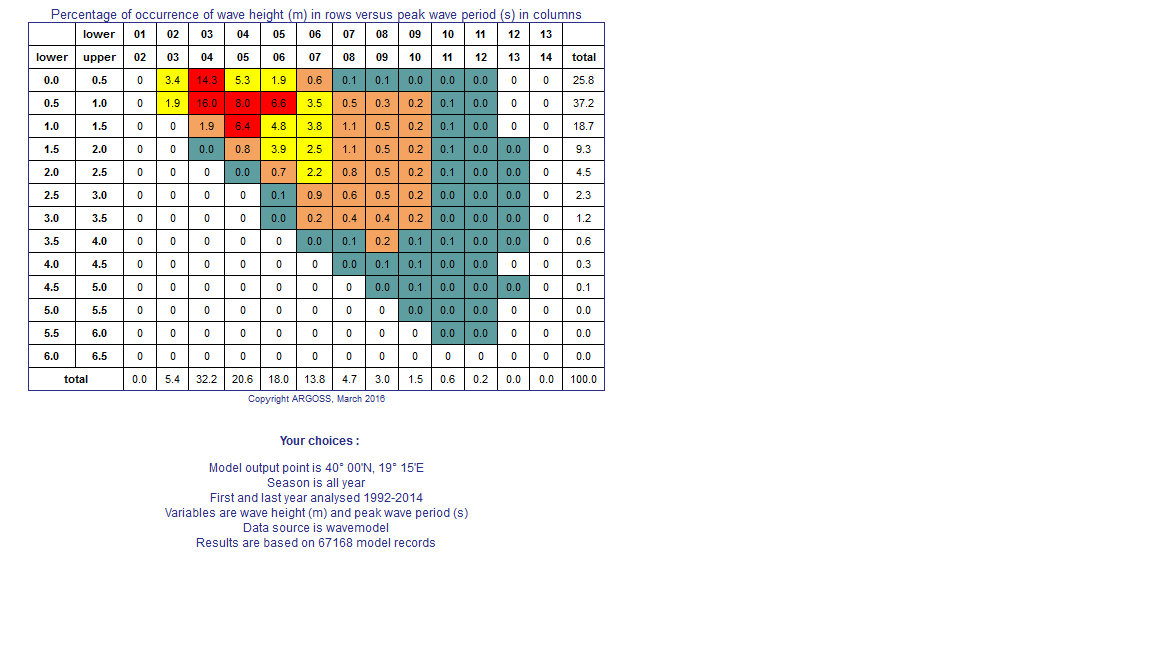
\includegraphics[width=\textwidth]{images/wave_pperiod_allyear.png} 
}
\caption[Distribution of peak-period over wave hight]{Distribution of peak-period over wave hight}
 %\label{Distribution_pperiod}
\end{figure}
% 
% 
\begin{figure}[H]
\center
\fbox{
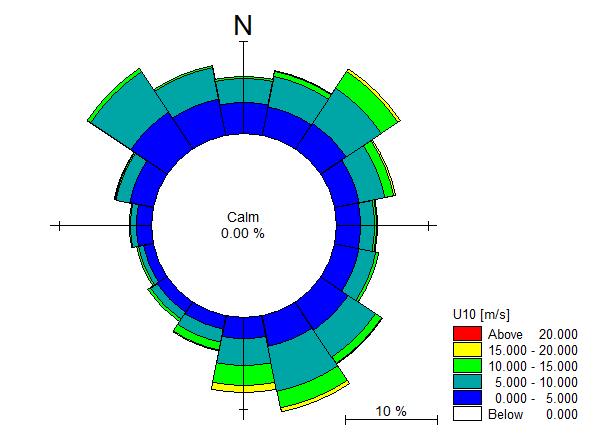
\includegraphics[width=\textwidth]{images/Rose_plot_u10.png} 
}
\caption{Rose-diagram with the distribution of the wind}
 %\label{Windrose}
\end{figure}
% 
% 
\begin{figure}[H]
\center
\fbox{
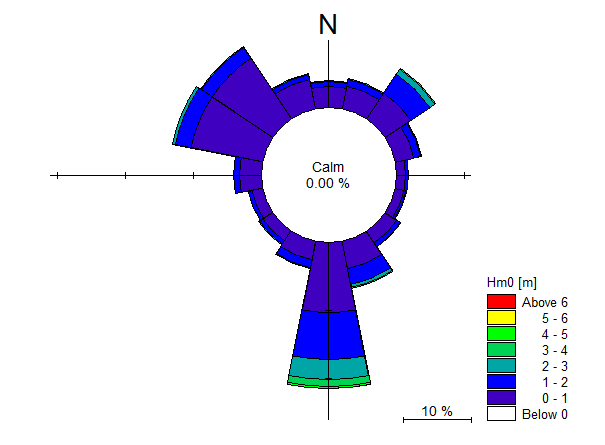
\includegraphics[width=\textwidth]{images/Rose_plot_Hoverall.png} 
}
\caption{Rose-diagram with the distribution of the waves}
% %\label{wavedata_angle}
\end{figure}

Whatever XX
